\documentclass[aspectratio=169,10pt]{beamer}

% -------------------------------------------------
% PACKAGES
% -------------------------------------------------

\usepackage[T1]{fontenc}
\usepackage{lmodern}
\usepackage{graphicx}
\usepackage{xcolor}
\usepackage{tikz}
\usepackage{booktabs}
\usepackage{tabularx}
\usepackage{array}

\usetikzlibrary{positioning,arrows.meta}

% -------------------------------------------------
% COLOURS
% -------------------------------------------------

\definecolor{GEUBlue}{RGB}{20,55,105}
\definecolor{GEULightBlue}{RGB}{238,244,251}
\definecolor{GEUGrey}{RGB}{90,90,90}

% -------------------------------------------------
% BEAMER SETTINGS
% -------------------------------------------------

\usetheme{default}

\setbeamertemplate{navigation symbols}{}

\setbeamercolor{normal text}{fg=black,bg=white}
\setbeamercolor{frametitle}{fg=GEUBlue}
\setbeamercolor{structure}{fg=GEUBlue}

\setbeamercolor{block title}{
    fg=GEUBlue,
    bg=GEULightBlue
}

\setbeamercolor{block body}{
    fg=black,
    bg=GEULightBlue
}

\setbeamerfont{frametitle}{
    size=\Large,
    series=\bfseries
}

% -------------------------------------------------
% GRAPHIC ERA LOGO
% -------------------------------------------------

% Upload graphicera_logo.png to the same Overleaf project.

\newcommand{\GEULogo}{graphicera_logo.png}

% -------------------------------------------------
% FRAME TITLE
% -------------------------------------------------

\setbeamertemplate{frametitle}{
    \vspace{0.2cm}
    \insertframetitle\par
    \vspace{0.08cm}
    \textcolor{GEUBlue}{\rule{\textwidth}{0.8pt}}
}

% -------------------------------------------------
% ABSOLUTE LOGO ON EVERY NORMAL SLIDE
% -------------------------------------------------

% The logo is positioned relative to the physical page.
% It does NOT reserve any space in the slide layout.

\setbeamertemplate{background}{%
    \begin{tikzpicture}[remember picture,overlay]
        \node[
            anchor=north east,
            inner sep=0pt,
            xshift=-0.30cm,
            yshift=-0.12cm
        ] at (current page.north east)
        {
            \includegraphics[height=1cm]{\GEULogo}
        };
    \end{tikzpicture}%
}

% -------------------------------------------------
% FOOTER
% -------------------------------------------------

\setbeamertemplate{footline}{
    \leavevmode
    \hbox{
        \begin{beamercolorbox}[
            wd=0.82\paperwidth,
            ht=0.32cm,
            dp=0.1cm,
            leftskip=0.3cm
        ]{author in head/foot}
        \tiny
        Department of Computer Science \& Engineering |
        Graphic Era (Deemed to be University)
        \end{beamercolorbox}
        %
        \begin{beamercolorbox}[
            wd=0.18\paperwidth,
            ht=0.32cm,
            dp=0.1cm,
            rightskip=0.3cm
        ]{date in head/foot}
        \hfill
        \tiny
        \insertframenumber/\inserttotalframenumber
        \end{beamercolorbox}
    }
}

% =================================================
% DOCUMENT INFORMATION
% =================================================

\title{Project-Based Learning}
\subtitle{Phase-I Evaluation}

\author{
    \textbf{MemDB}\\
    Team ID: DSCPP-III-2026-T229
}

\institute{
    Department of Computer Science \& Engineering\\
    Graphic Era (Deemed to be University), Dehradun
}

\date{Academic Session 2026--27}

% =================================================
% DOCUMENT
% =================================================

\begin{document}

% -------------------------------------------------
% SLIDE 1 - TITLE
% -------------------------------------------------

\begin{frame}[plain]

\begin{tikzpicture}[remember picture,overlay]


% -------------------------------------------------
% TOP LINE
% -------------------------------------------------

\draw[
    GEUBlue,
    line width=3pt
]
(current page.north west)
--
(current page.north east);

% -------------------------------------------------
% MAIN TITLE
% -------------------------------------------------

\node[
    align=center,
    text width=0.85\paperwidth
]
at ([yshift=0.3cm]current page.center)
{

{\color{GEUBlue}
\fontsize{26}{30}
\selectfont
\bfseries
PROJECT-BASED LEARNING}

\\[4mm]

{\fontsize{18}{22}
\selectfont
PHASE-I EVALUATION}

\\[8mm]

{\color{GEUGrey}
\fontsize{20}{24}
\selectfont
\bfseries
MemDB: In-Memory Key-Value Cache}

\\[3mm]

{\color{GEUBlue}
\large
Team ID: DSCPP-III-2026-T229}

};

% -------------------------------------------------
% UNIVERSITY INFORMATION
% -------------------------------------------------

\node[
    align=center,
    anchor=south
]
at ([yshift=0.5cm]current page.south)
{

\bfseries
Department of Computer Science \& Engineering

\\[1mm]

Graphic Era (Deemed to be University), Dehradun

\\[1mm]

\scriptsize
Academic Session 2026--27

};

\end{tikzpicture}

\end{frame}


% -------------------------------------------------
% SLIDE 2 - TEAM
% -------------------------------------------------

\begin{frame}{Team \& Mentor Details}

\begin{columns}[T]

% LEFT
\begin{column}{0.48\textwidth}

\begin{block}{Team Information}

\begin{tabular}{@{}ll@{}}

\textbf{Team ID:} & DSCPP-III-2026-T229 \\[2mm]

\textbf{Semester:} & 3rd \\[2mm]

\textbf{Domain:} & Systems / Software \\[2mm]

\textbf{Project:} & MemDB

\end{tabular}

\end{block}

\end{column}

% RIGHT
\begin{column}{0.48\textwidth}

\begin{block}{Team Members}

\small

1. Anish Mandal (ML1) -- 2028642

\vspace{2mm}

2. Arnav Rawat (ML4) -- 2028398

\vspace{2mm}

3. Priyanshi (DS2) -- 2028468

\vspace{2mm}

4. Suhani Rawat (DS1) -- 2028504

\end{block}

\end{column}

\end{columns}

\vspace{3mm}

\begin{block}{Mentor}

\textbf{Dr. Ravi Sharma}

\hfill

\textbf{Number of Interactions: 2}

\end{block}

\vspace{2mm}

\small
\textcolor{GEUGrey}{
Arnav Rawat is the team lead.
}

\end{frame}


% -------------------------------------------------
% SLIDE 3 - PROBLEM STATEMENT & MOTIVATION
% -------------------------------------------------

\begin{frame}{Problem Statement \& Motivation}

\small

\begin{block}{Problem Statement}

Applications often access the same data repeatedly. Fetching data from
slower storage can increase access time. MemDB provides a lightweight
\textbf{in-memory key-value cache} that keeps frequently accessed data
in memory while managing lookup, capacity, expiration and eviction.

\end{block}

\vspace{2mm}

\begin{columns}[T]

\begin{column}{0.48\textwidth}

\textbf{\color{GEUBlue}Why MemDB?}

\begin{itemize}
    \itemsep2pt
    \item Reduce repeated data access.
    \item Understand caching internally.
    \item Apply data structures to a real problem.
    \item Study cache eviction strategies.
    \item Measure performance using benchmarks.
\end{itemize}

\end{column}

\begin{column}{0.48\textwidth}

\textbf{\color{GEUBlue}Project Focus}

\begin{itemize}
    \itemsep2pt
    \item Hash-based key lookup.
    \item Linked-list collision handling.
    \item LRU and FIFO eviction.
    \item TTL-based expiration.
    \item Memory and cache statistics.
\end{itemize}

\end{column}

\end{columns}

\vspace{1mm}

\begin{center}

\colorbox{GEULightBlue}{
\parbox{0.78\textwidth}{
\centering
\textbf{\color{GEUBlue}Goal:}
Build and evaluate a lightweight in-memory cache using
fundamental data structures and cache policies.
}}

\end{center}

\end{frame}


% -------------------------------------------------
% SLIDE 4 - OBJECTIVES
% -------------------------------------------------

\begin{frame}{Objectives}

\textbf{\color{GEUBlue}Project Objectives}

\vspace{2mm}

\begin{enumerate}

\item Develop a functional lightweight in-memory key-value cache.

\item Implement hash-based key lookup with collision handling.

\item Implement LRU and FIFO cache eviction policies.

\item Implement TTL-based expiration using a min-heap.

\item Apply C data structures and C++ object-oriented abstractions.

\item Track memory usage and cache statistics.

\item Evaluate the implementation using controlled workloads
and measurable metrics.

\end{enumerate}

\vfill

\begin{center}

\colorbox{GEULightBlue}{
\parbox{0.82\textwidth}{
\centering

\textbf{\color{GEUBlue}Key Objective}

\vspace{1mm}

Build and experimentally evaluate a lightweight in-memory cache
using explicitly implemented data structures and cache policies.

}}

\end{center}

\end{frame}


% -------------------------------------------------
% SLIDE 5 - PROPOSED SOLUTION
% -------------------------------------------------

\begin{frame}{Proposed Solution}

\begin{columns}[T]

\begin{column}{0.48\textwidth}

\textbf{\color{GEUBlue}Approach}

\begin{enumerate}

\item Store key-value entries in memory.

\item Use a hash table for average $O(1)$ key lookup.

\item Handle collisions using linked lists.

\item Maintain order for eviction policies.

\item Use a min-heap for earliest TTL expiration.

\item Track memory consumption and statistics.

\item Provide a C++ interface over the structures.

\end{enumerate}

\end{column}

\begin{column}{0.48\textwidth}

\textbf{\color{GEUBlue}Core Features}

\begin{itemize}

\item SET / GET

\item DELETE / CLEAR

\item LRU eviction

\item FIFO eviction

\item TTL expiration

\item Configurable capacity

\item Hit / miss statistics

\item Memory usage tracking

\item Benchmarking

\end{itemize}

\end{column}

\end{columns}

\vfill

\small
\textcolor{GEUGrey}{
The listed features form the proposed implementation scope.
}

\end{frame}


% -------------------------------------------------
% SLIDE 6 - PBL INTEGRATION
% -------------------------------------------------

\begin{frame}{Integration of PBL Course Concepts}

\begin{block}{Data Structures in C}

Hash tables, linked lists, doubly linked lists, min-heaps and
dynamic memory management support cache storage, collision
handling, LRU ordering and TTL management.

\end{block}

\vspace{3mm}

\begin{block}{OOPs with C++}

Classes, encapsulation, abstraction and polymorphism organize
cache management and eviction-policy implementations.

\end{block}

\vfill

\begin{center}

\colorbox{GEULightBlue}{
\parbox{0.82\textwidth}{
\centering

\textbf{\color{GEUBlue}Integration}

C provides low-level data structures, while C++ provides
higher-level cache management and policy abstraction.

}}

\end{center}

\end{frame}


% -------------------------------------------------
% SLIDE 7 - ARCHITECTURE
% -------------------------------------------------

\begin{frame}{System Architecture / Workflow}

\begin{center}

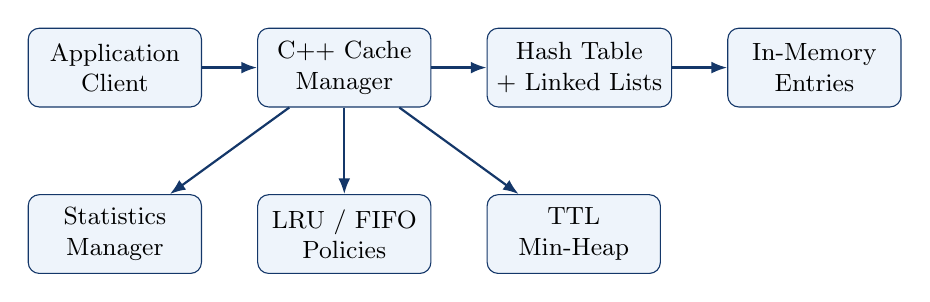
\begin{tikzpicture}[
    box/.style={
        rectangle,
        rounded corners,
        draw=GEUBlue,
        fill=GEULightBlue,
        minimum width=2.2cm,
        minimum height=1cm,
        align=center,
        font=\small
    },
    arrow/.style={
        -{Latex[length=2mm]},
        thick,
        draw=GEUBlue
    }
]

\node[box] (app)
{Application\\Client};

\node[box,right=0.7cm of app] (manager)
{C++ Cache\\Manager};

\node[box,right=0.7cm of manager] (hash)
{Hash Table\\+ Linked Lists};

\node[box,right=0.7cm of hash] (memory)
{In-Memory\\Entries};

\draw[arrow]
(app) -- (manager);

\draw[arrow]
(manager) -- (hash);

\draw[arrow]
(hash) -- (memory);

\node[box,below=1.1cm of manager] (policy)
{LRU / FIFO\\Policies};

\node[box,right=0.7cm of policy] (ttl)
{TTL\\Min-Heap};

\node[box,left=0.7cm of policy] (stats)
{Statistics\\Manager};

\draw[arrow]
(manager) -- (policy);

\draw[arrow]
(manager) -- (ttl);

\draw[arrow]
(manager) -- (stats);

\end{tikzpicture}

\end{center}

\vspace{4mm}

\begin{columns}[T]

\begin{column}{0.48\textwidth}

\textbf{\color{GEUBlue}Core Components}

\begin{itemize}

\item Hash table
\item Collision lists
\item LRU / FIFO policies
\item TTL min-heap
\item Statistics

\end{itemize}

\end{column}

\begin{column}{0.48\textwidth}

\textbf{\color{GEUBlue}Workflow}

\begin{itemize}

\item Application sends GET / SET.
\item Hash table locates the entry.
\item Policy state is updated.
\item TTL manager tracks expiration.
\item Statistics are recorded.

\end{itemize}

\end{column}

\end{columns}

\end{frame}


% -------------------------------------------------
% SLIDE 8 - TECHNOLOGY
% -------------------------------------------------

\begin{frame}{Technology Stack \& Methodology}

\begin{columns}[T]

\begin{column}{0.48\textwidth}

\begin{block}{Technology Stack}

\begin{itemize}

\item Programming: C and C++

\item Core data structures: C

\item Cache management / OOP: C++

\item Development environment: Windows

\item Version control: Git / GitHub

\item Testing: Custom test programs and workloads

\end{itemize}

\end{block}

\end{column}

\begin{column}{0.48\textwidth}

\begin{block}{Development Methodology}

\begin{enumerate}

\item Requirement analysis

\item Data structure design

\item Cache architecture

\item Core implementation

\item Policy and TTL implementation

\item Testing

\item Benchmarking

\item Evaluation

\end{enumerate}

\end{block}

\end{column}

\end{columns}

\vfill

\begin{center}

\small
\textcolor{GEUGrey}{
The project focuses on the in-memory cache and its underlying
algorithms and data structures.
}

\end{center}

\end{frame}


% -------------------------------------------------
% SLIDE 9 - PROGRESS
% -------------------------------------------------

\begin{frame}{Initial Progress \& Team Contribution}

\begin{columns}[T]

\begin{column}{0.45\textwidth}

\textbf{\color{GEUBlue}Progress Achieved}

\begin{itemize}

\item Problem and scope identified.

\item Core cache operations defined.

\item Hash table selected for lookup.

\item Linked lists selected for collisions.

\item Doubly linked list selected for LRU.

\item Min-heap selected for TTL.

\item LRU and FIFO selected as policies.

\item Benchmarking metrics identified.

\end{itemize}

\end{column}

\begin{column}{0.52\textwidth}

\textbf{\color{GEUBlue}Team Contribution}

\vspace{2mm}

\scriptsize

\begin{tabularx}{\textwidth}{
    @{}
    >{\raggedright\arraybackslash}p{1.45cm}
    >{\raggedright\arraybackslash}p{1.35cm}
    X
    @{}
}

\toprule

Member & Role & Contribution \\

\midrule

Anish Mandal &
Developer &
Core implementation, data structures and system design \\

Arnav Rawat &
Team Lead &
Coordination, architecture and implementation \\

Priyanshi &
Developer &
Testing, cache operations and evaluation \\

Suhani Rawat &
Developer / Documentation &
Documentation, testing and project support \\

\bottomrule

\end{tabularx}

\end{column}

\end{columns}

\end{frame}


% -------------------------------------------------
% SLIDE 10 - ROADMAP
% -------------------------------------------------

\begin{frame}
{Roadmap, Outcomes \& References}

\begin{columns}[T]

\begin{column}{0.47\textwidth}

\textbf{\color{GEUBlue}Roadmap}

\begin{enumerate}

\item Phase-I: Requirements \& architecture

\item Phase-II: Core data structures

\item Phase-III: LRU, FIFO \& TTL

\item Phase-IV: Testing \& benchmarking

\item Phase-V: Visualization \& evaluation

\end{enumerate}

\vspace{3mm}

\textbf{\color{GEUBlue}Expected Outcomes}

\begin{itemize}

\item Working in-memory cache

\item DSA implementation in C

\item OOP-based management in C++

\item LRU, FIFO and TTL

\item Statistics and memory tracking

\item Benchmark results

\end{itemize}

\end{column}

\begin{column}{0.47\textwidth}

\textbf{\color{GEUBlue}References}

\begin{enumerate}

\item Cormen et al.,
\textit{Introduction to Algorithms}

\item Kernighan \& Ritchie,
\textit{The C Programming Language}

\item Bjarne Stroustrup,
\textit{The C++ Programming Language}

\end{enumerate}

\vfill

\begin{center}

\colorbox{GEUBlue}{
\parbox{0.75\textwidth}{
\centering

\color{white}

\textbf{Thank You}

\\[1mm]

Questions \& Suggestions

}}

\end{center}

\end{column}

\end{columns}

\end{frame}


% -------------------------------------------------
% END
% -------------------------------------------------

\end{document}